\documentclass[a4j,12pt]{jsarticle}
\usepackage{semi}
\begin{document}

\newpage
\section{緒言}


各塾の調査では中学,高校で学習する科目の中で数学と英語は苦手になりやすいと言われている\cite{1}.この2科目の共通点である積み上げ型教科という点に注目した.科目には独立型教科と積み上げ型教科の2種類に分けられると言われている.独立型教科とは単元ごとに独立していて,単元ごとの関連性があまりない教科を指し,どの単元から学習しても支障が出ない.それに対して積み上げ型教科とは既に学習した知識を使うことを前提として次の単元を学習する教科で,ある程度決められた順番で学習する必要がある.本研究では前提知識となる単元を「前提単元」,前提知識を用いて学習を行う単元を「主単元」と称した.前提単元には学習目的が主単元で利用することになっているものがあり,このような単元は学習目的や実用例などのイメージがしづらく,理解の妨げになっていると考えた.また前提単元が理解できないと主単元にまで影響を及ぼしてしまい,理解できない単元が増えるため,苦手な教科になってしまう.

そこで前提単元の具体例がわかりづらく,主単元の具体例がわかりやすいときに限り,「主単元の概要をあらかじめ学習することで,前提単元の理解を促進することができる」という仮説を立てた.

本研究では,積み上げ型教科の理解力向上を目的として,講義にて学生を対象に実験を行い,この仮説を検証する.

\newpage
\section{教科の特性}
学校で学習する教科には独立型教科と積み上げ型教科に分かれ,積み木のような図で表される.\\


\subsection{独立型教科}
独立型教科とは単元ごとに独立していて,単元ごとの関連性があまりない教科を指し,主に国語や社会が該当する.
図\ref{fig:01}は社会の単元である「地理」「歴史」「公民」がそれぞれ独立していることを示している.

独立している各単元の中で積み上げ型教科の特性を示しているものや,独立している各単元で繋がりがあることもあるが,
基本的にはどの単元から学習しても支障がない.\\
\begin{figure}[H]
\centering
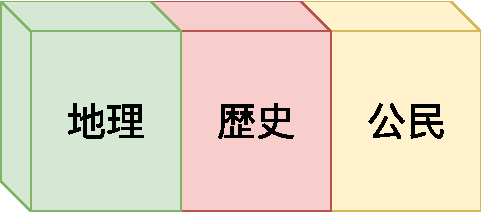
\includegraphics[width=6cm]{01.pdf}
\caption{独立型教科の例}
\label{fig:01}
\end{figure} 

\newpage
\subsection{積み上げ型教科}
積み上げ型教科とは既に学習した知識を使うことを前提として次の単元を学習する教科で,主に数学や英語が該当する.
図\ref{fig:04}では数学を例としてあげている.この例ではまず「正の数・負の数」を学習し,それを前提単元として「文字式」を学習する.
次に学習した「文字式」を前提単元として「方程式」や「平面図形」を学習する.
「方程式」「平面図形」をそれぞれ前提単元として「比例・反比例」「空間図形」を学習していく..
積み上げ型教科ではこのように学習した内容を次の学習の基礎知識として用いるため,順番に学習していくことになる.\\

\begin{figure}[H]
\centering
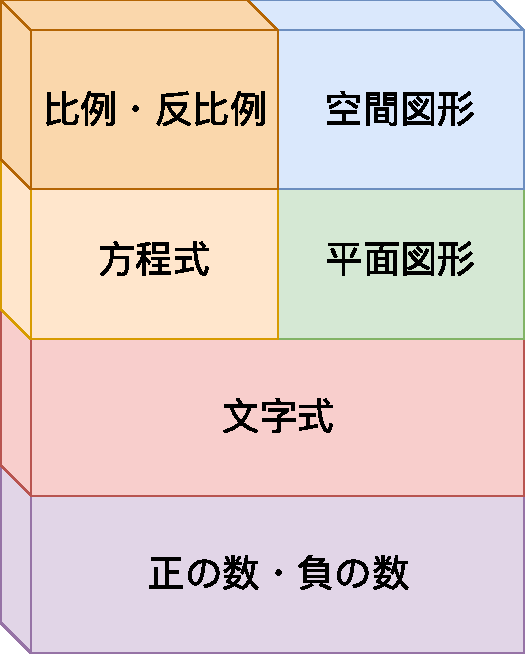
\includegraphics[width=4cm]{04.pdf}
\caption{積み上げ型教科の例}
\label{fig:04}
\end{figure} 
\ \\
積み上げ型教科には大きく分けて3種類の形が存在する.図\ref{fig:03}では3種類の形を示す.

左側の図は1つの前提単元を用いて,1つの主単元を学習する形を表した図である.
中央の図は1つの前提単元を用いて,複数の主単元を学習する形を表した図である.
右側の図は複数の前提単元を用いて1つの主単元を学習する形を表した図である.
\begin{figure}[H]
\centering
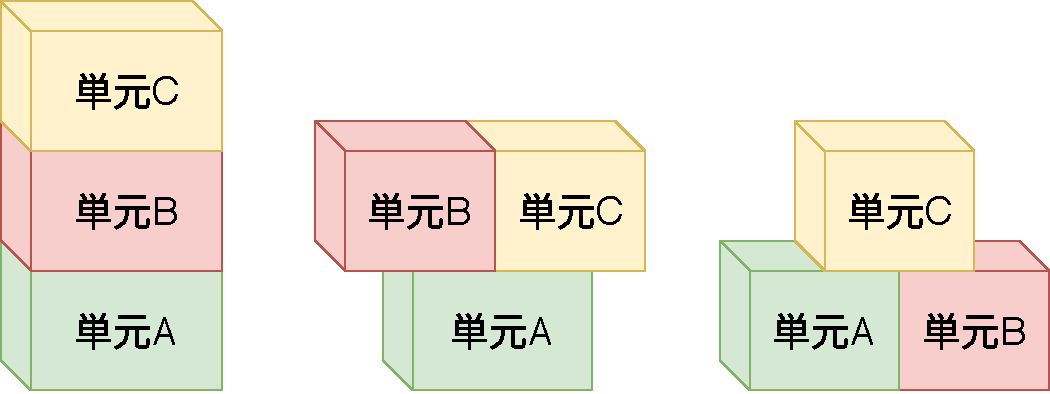
\includegraphics[width=12cm]{03.pdf}
\caption{積み上げ型教科の教育モデル}
\label{fig:03}
\end{figure} 




\newpage
\section{ハッシュ関数}

任意のデータを固定長の値であるハッシュ値に置き換える関数である.
ハッシュ関数は不可逆的な一方向関数であり,ハッシュ値から元のデータに復元することは不可能である.

\begin{figure}[H]
\centering
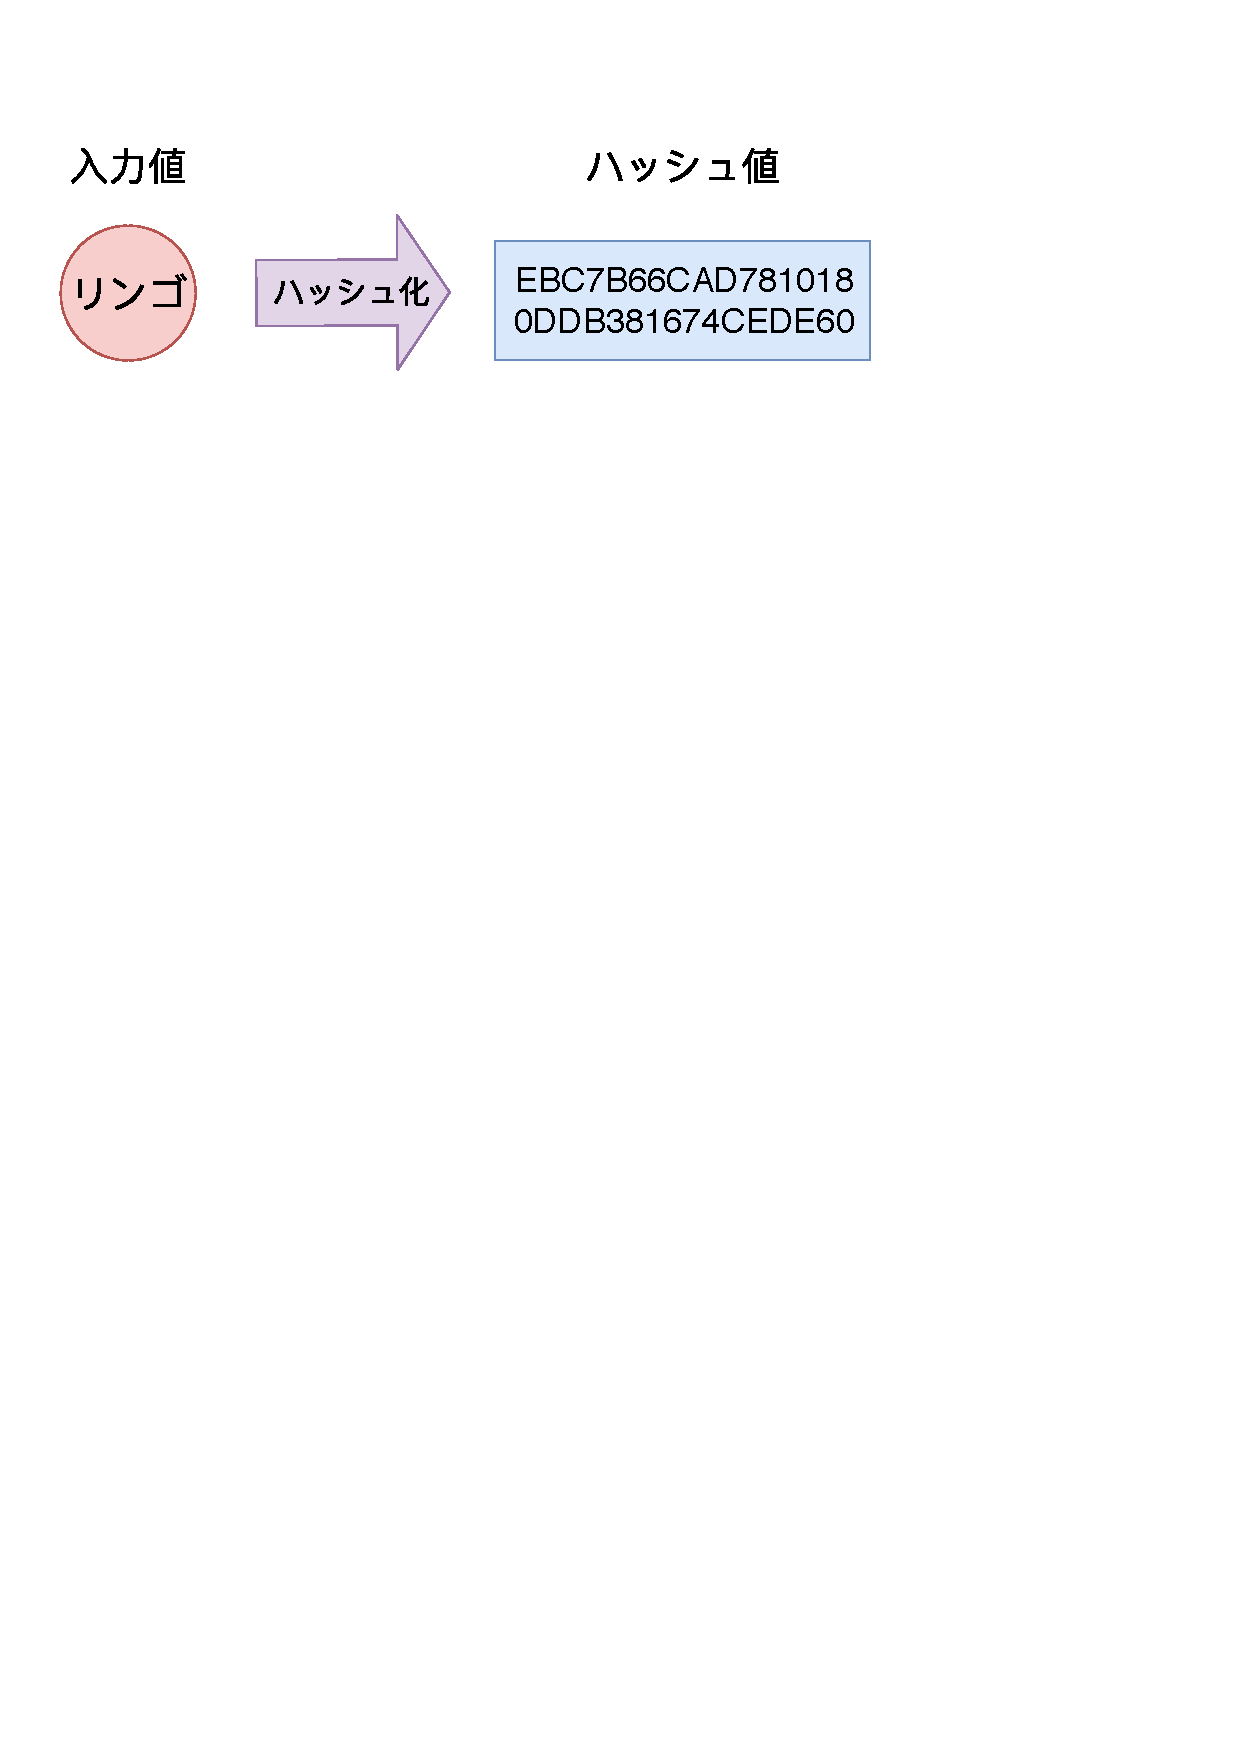
\includegraphics[mediaboxonly=/CropBox,width=12cm]{hash1.pdf}
\caption{ハッシュ化の例}
\label{fig:01}
\end{figure} 


\subsection {ハッシュ関数の安全性}
ハッシュ関数の安全性について以下の3種類の特徴がある.
\begin{description}
\item[衝突困難性(強衝突耐性)]\ \\
同じハッシュ値を与える2つの入力値を求めることが困難であるような性質である.

\item[第二原像計算困難性(弱衝突耐性)]\ \\ 
与えられた入力値に対して,その入力値のハッシュ値と同じハッシュ値の入力値を求めることが困難であるような性質である.

\item[原像計算困難性]\ \\
与えられたハッシュ値に対して,そのハッシュ値を出力する入力値を求めることが困難であるような性質である.
\end{description}

一つのアルゴリズムについて違う入力値の同じハッシュ値が見つかることを強衝突耐性の突破と呼び,
与えられた入力値と同じハッシュ値の入力値を求められるようになることを弱衝突耐性の突破と呼ぶ.

原像計算困難性を満たさないハッシュ関数では,任意の入力値からハッシュ値を得られるため,第二原像困難性を満たさない.
また第二原像計算困難性を満たさないハッシュ関数では,衝突困難性を満たさない.
したがって,

原像計算困難性 ⊃ 第2原像計算困難 ⊃ 衝突困難

である.



\newpage
\subsection {ハッシュ関数のアルゴリズム}
ハッシュ関数はハッシュ値のビット数や,仕組みによって様々な種類がある.
以下はハッシュ関数の中でも代表的なアルゴリズムである.


\begin{description}
\item[MD5]\ \\
1991年に開発されたハッシュ値が128ビットのハッシュ関数の一つである.
それほど性能の高くないコンピュータでも數十分程度で同一ハッシュ値のデータ列が生成できるため,強衝突耐性が容易に突破される状態にある.しかし弱衝突耐性は容易に突破されることはない.


\item[SHA-1]\ \\ 
ハッシュ値が160ビットのSecure Hash Algorithm(SHA)シリーズのハッシュ関数の一つである.
アメリカ合州国において機密情報を扱う際に法律によって要求されるハッシュアルゴリズムとして用いられていたが,2011年に理論上ではあるが強衝突耐性を突破されているため,改良版であるSHA-2へ移行している.

\item[SHA-2]\ \\
SHA-1が改良されて作られたハッシュ関数で,SHA-224,SHA-256,SHA-384,SHA-512と呼ばれるハッシュ関数の総称である.またビット数はそれぞれ224ビット,256ビット,384ビット,512ビットであり,SHA-1より長くなっている.
その中でもSHA-256は計算速度や安全性のバランスに優れていて,もっとも普及している.ビットコインに使われているのもSHA-256である.
\end{description}



\newpage
\subsection {ハッシュ関数の実用例}
\subsubsection{ファイルの同一性確認}


ハッシュ関数は改ざんや破損の検知など,ファイルの同一性確認に使用される.

図\ref{fig:hash1}は2つのハッシュ値を比較して一致した時と不一致の時の図である.

\begin{figure}[H]
\centering
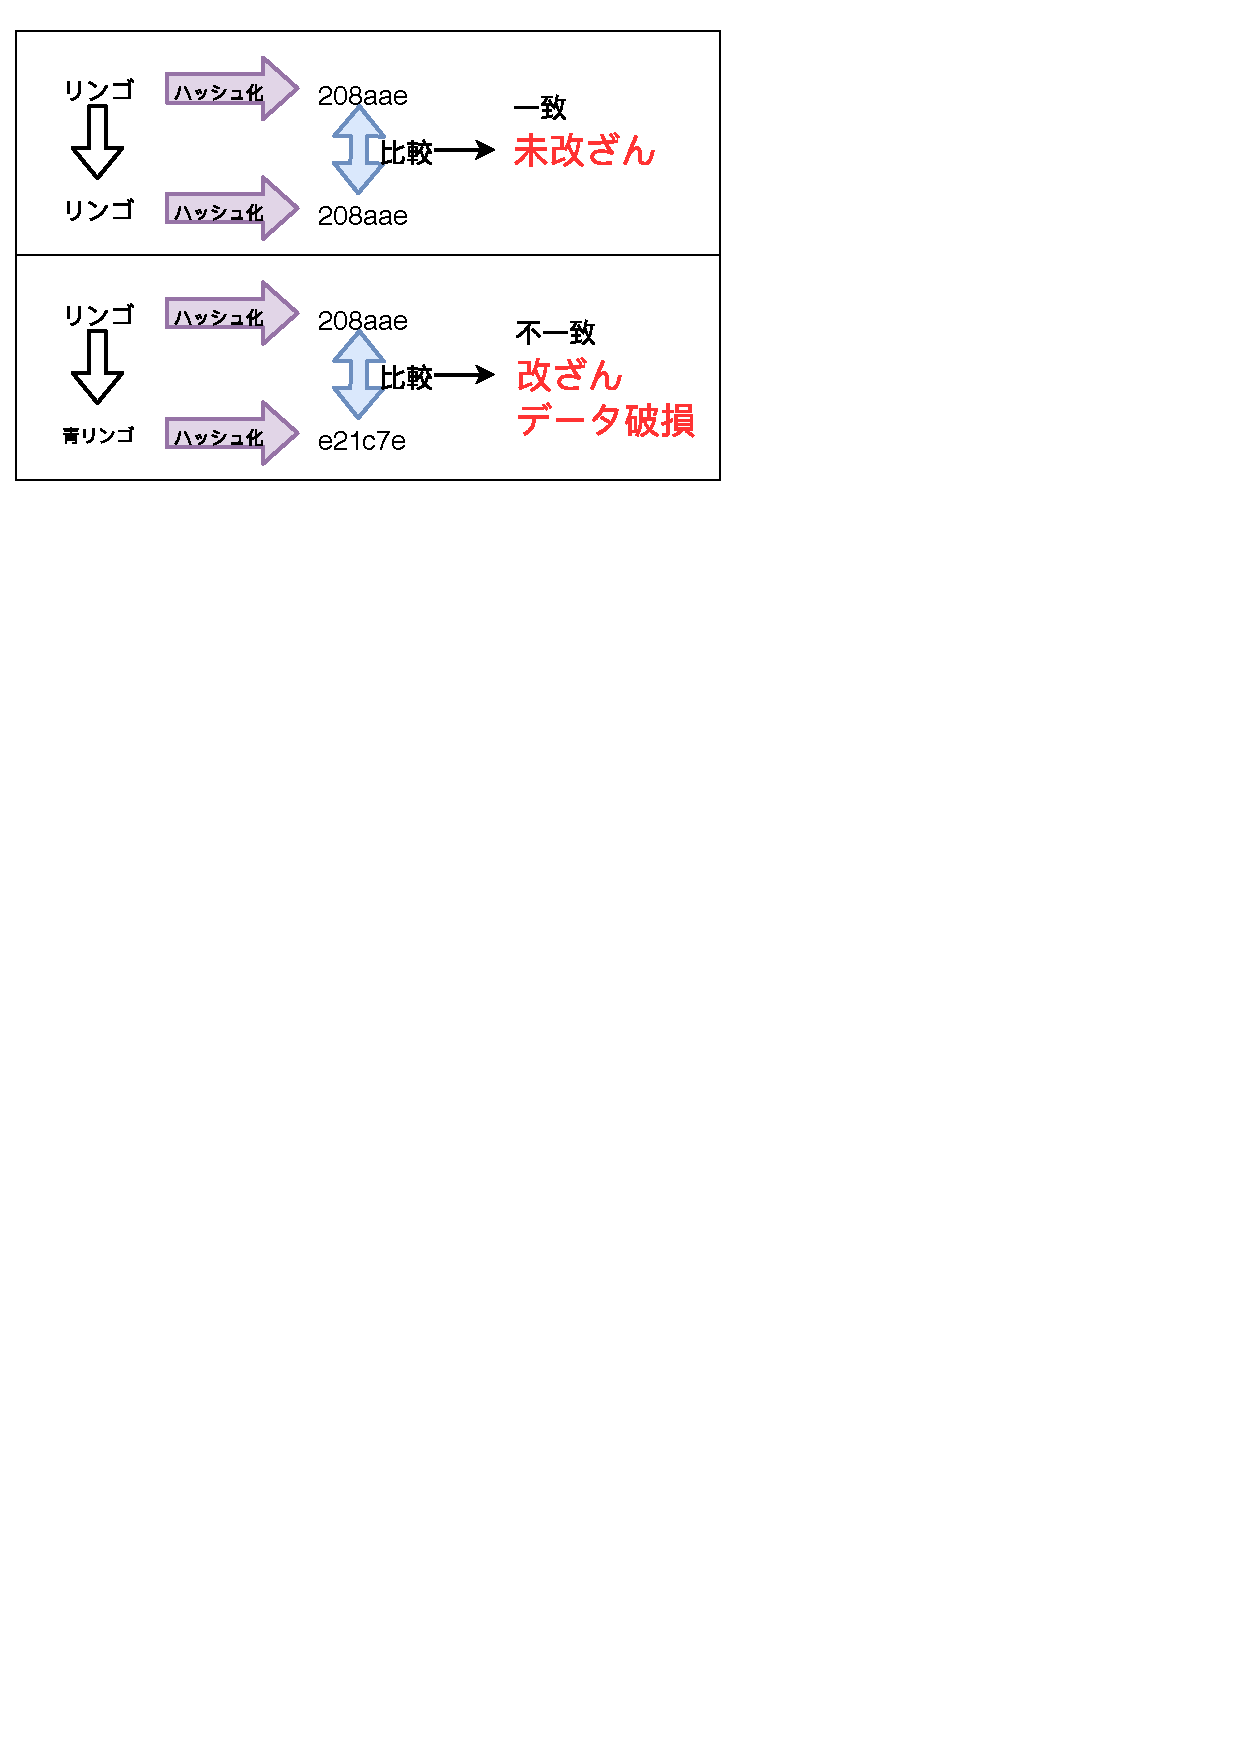
\includegraphics[width=11cm]{hash.pdf}
\caption{ハッシュを用いたファイルの同一性確認の流れ}
\label{fig:hash1}
\end{figure} 

\subsubsection{パスワードの管理}
ハッシュ関数はWEBサイトなどでパスワードを用いる際に使われる.パスワードを平文で管理するとパスワードが漏洩したときに第三者に不正にアクセスされる危険がある.そのためパスワードをハッシュ化し,ハッシュ値の状態で管理することで漏洩しても不正ログインを防ぐことができる.

しかし同じデータをハッシュ化すると同じハッシュ値になることから,あらかじめ使われやすい単語などをハッシュ化しデータベース化し,不正ログインを試みようとするサイトがある.そのため以下のような手段が取られている.

\begin{description}
\item[saltを加える]\ \\
平文のパスワードにsaltと呼ばれるランダムな文字列を加えることによって,1つの文字列に対するハッシュ値の種類を増やすことで,データベースを作成しておく攻撃を困難にする.

\item[ハッシュ関数を繰り返す]\ \\ 
平文のパスワードをハッシュ化して出たハッシュ値を,さらにハッシュ化することによって新たなハッシュ値を生成することができる.

\end{description}




\newpage
\section{暗号}
暗号とは通信を行う際,第三者にその内容を知られないようにするための手段である.
元の文に一定の規則を用いて特定の変形を加えることを暗号化,暗号化する前の元の文を平文,暗号から平文に戻すことを復号と呼ぶ.
暗号化する手段が暗号アルゴリズムであり,また暗号化や復号化に使うデータを鍵と呼ぶ.
暗号は特性によって古典暗号と現代暗号に分かれる.
アルゴリズムがわかれば解読が容易になる暗号を古典暗号,アルゴリズムは公開するが鍵を非公開にすれば安全な暗号を現代暗号という.

\newpage
\subsection{共通鍵暗号}
暗号化と復号に同じ鍵を用いる暗号の方式である.
通信相手に鍵を送り,その鍵を用いて情報を暗号化する.
暗号化された情報が送られてきたら,同じ鍵を使って復号する.


\begin{figure}[H]
\centering
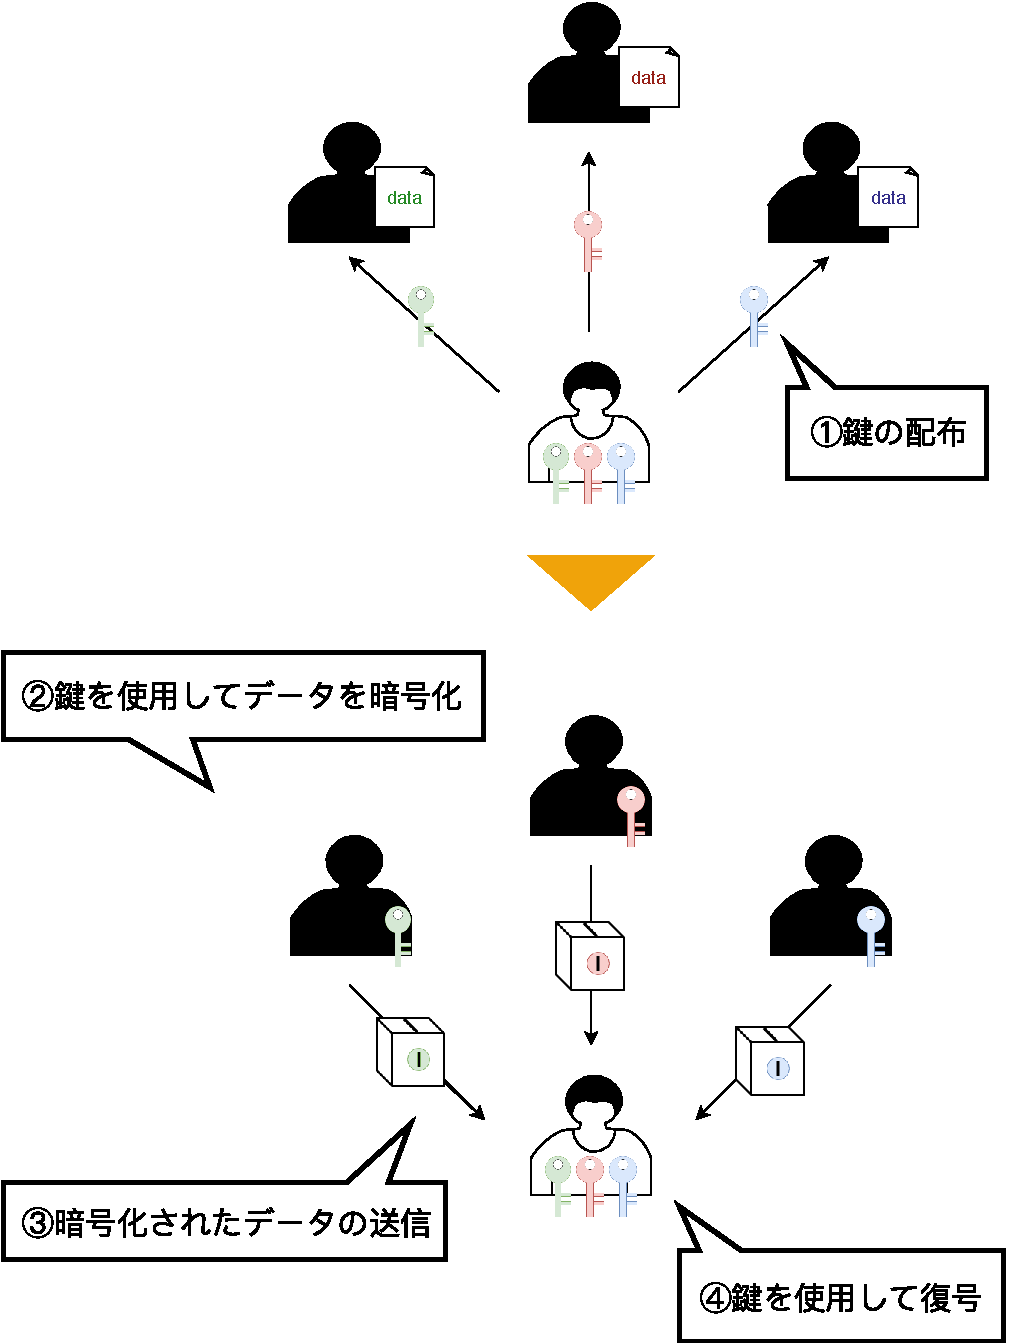
\includegraphics[width=10cm]{kyotu.pdf}
\caption{共通鍵暗号通信の流れ}
\label{fig:no}
\end{figure} 

共通鍵暗号通信では暗号化と同じ鍵を使っているため,鍵を送る際に第三者に傍受される危険がある.
また同じ鍵を複数のユーザーで使用すると,他のユーザーが復号する危険性があるため,ユーザーごとに鍵を生成する必要がある.

\newpage
\subsubsection{換字式暗号の仕組みと例}
平文の文字を他の記号や文字に置き換えて暗号文を作る古典暗号の方式である.
換字式暗号の代表としてシーザー暗号がある.
シーザー暗号は鍵である決められた文字数分のアルファベットをずらして暗号化を行う.
図\ref{fig:05}は鍵が1であるときの例である.\\

\begin{figure}[H]
\centering
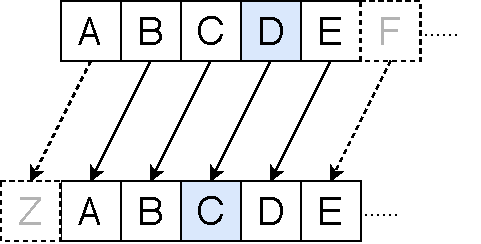
\includegraphics[width=9cm]{05.pdf}
\caption{シーザー暗号の例}
\label{fig:05}
\end{figure} 


\subsubsection{転置式暗号の仕組みと例}
平文の位置を並び替えて暗号文を作る古典暗号の方式である.
転置式暗号の代表としてスキュタレー暗号がある.
スキュタレー暗号はスキュタレーと呼ばれるシリンダーに細長い紙を巻きつけ,平文を横書きに書く.
紙をスキュタレーから外すと順番が入れ替わった暗号ができる.
暗号の受け取る側は同じ半径のスキュタレーを用意し,紙を巻きつけることで復号することができる.
この場合,鍵は同じ直径であることである.\\

\begin{figure}[H]
\centering
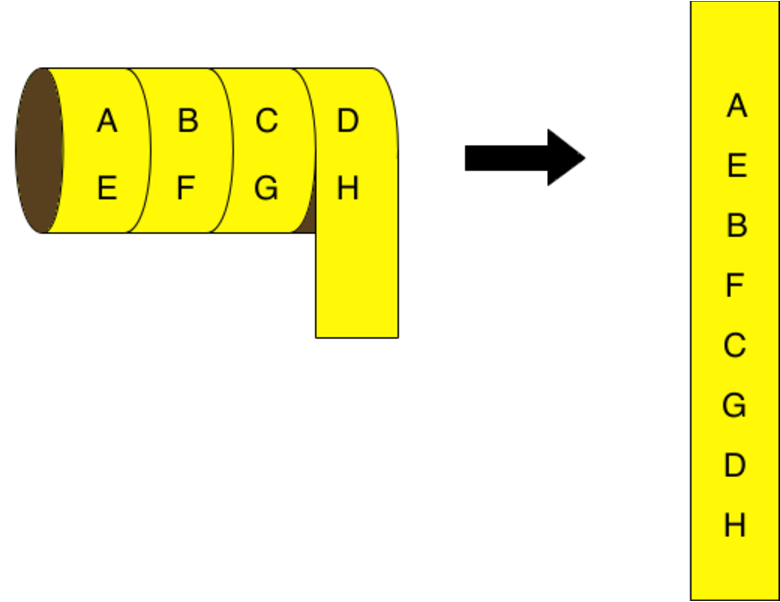
\includegraphics[width=8cm]{062.pdf}
\caption{スキュタレー暗号の例}
\label{fig:06}
\end{figure} 


\newpage
\subsection{公開鍵暗号}

暗号化と復号に別の手順を用いる暗号方式である.
ユーザは秘密鍵から公開鍵を生成する.
通信相手に送る鍵を公開鍵と呼び,自分の手元に保管しておく鍵を秘密鍵と呼ぶ.
公開鍵を通信相手に送り,通信相手は公開鍵を使って情報を暗号化する.
ユーザは受け取った暗号化された情報を秘密鍵を用いて復号する.

公開鍵暗号では「閉じることはできても開けることができないこと」を安全の根拠としており,一方向関数である素因数分解や楕円曲線が使われる.



\begin{figure}[H]
\centering
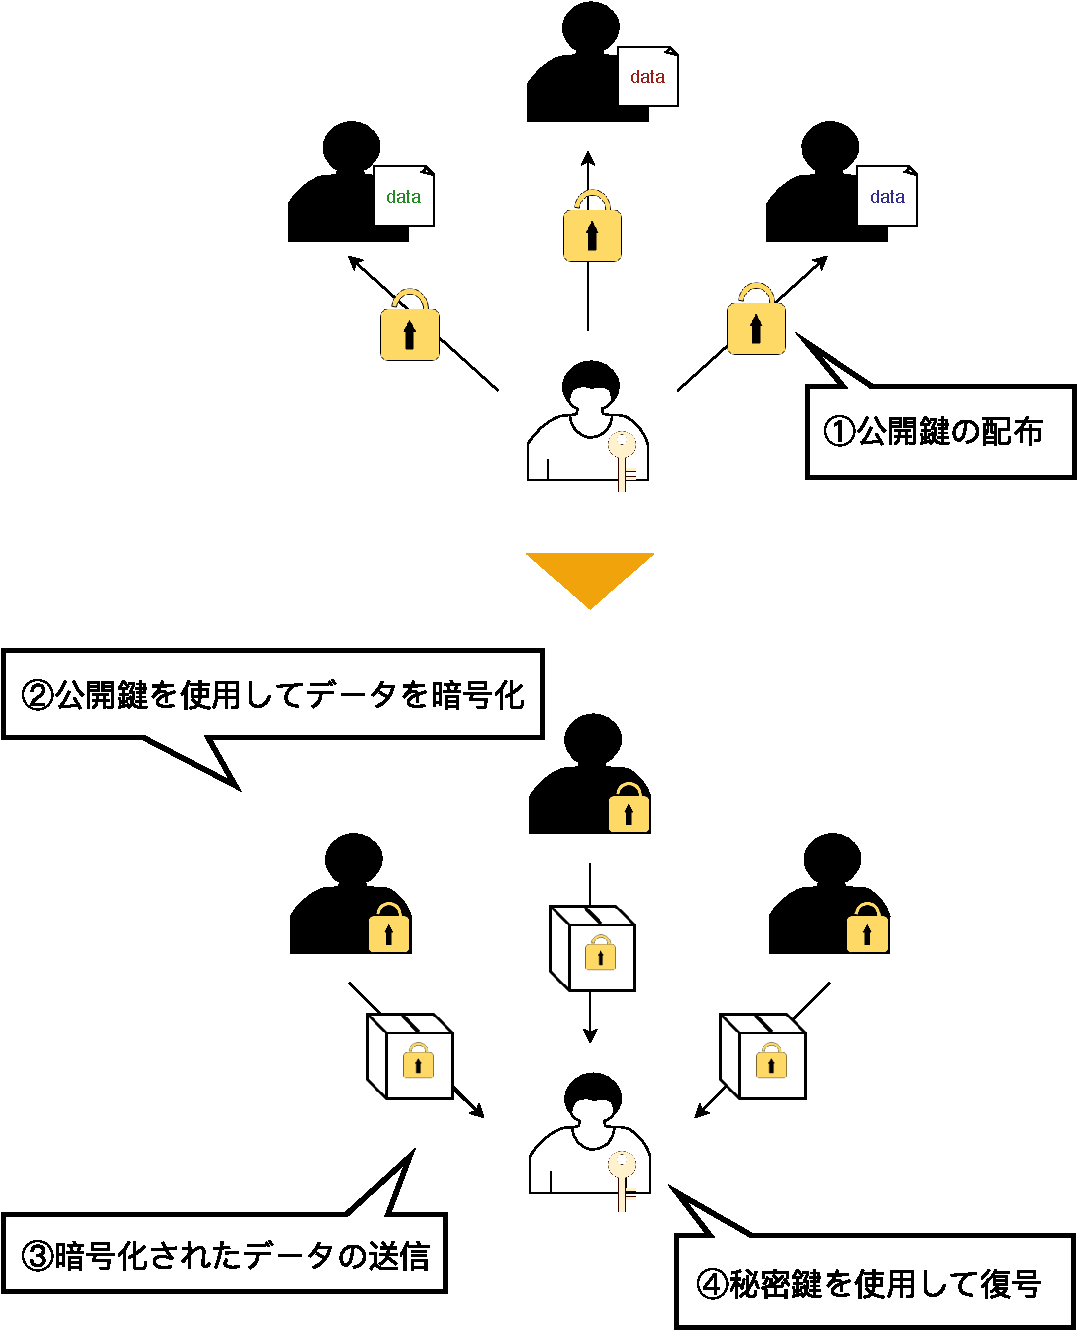
\includegraphics[width=10cm]{kokai.pdf}
\caption{公開鍵暗号通信の流れ}
\label{fig:no}
\end{figure} 

公開鍵暗号は共通鍵暗号とは違い各ユーザーごとに鍵を生成する必要がない.
また鍵の受け渡しの際に傍受される可能性がある共通鍵暗号通信とは違い,公開鍵では復号することができない.そのため共通鍵暗号通信よりも安全性が高い.しかし復号に複雑な計算を用いるため負荷が大きくなるため通信に時間がかかるという欠点もある.



\subsubsection{RSA暗号}
RSA暗号とは現在インターネットで広く使われている公開鍵暗号の一つである.
発明者であるRonald Linn Rivest,Adi Shamir,Leonard Max Adlemanの頭文字をとって名付けられた.
RSA暗号は桁数の多い素数の掛け算をするのは簡単だが,その合成数の素因数分解をするのは困難であることを安全性の根拠としている.


\subsubsection{電子署名の仕組み}

RSA暗号や楕円曲線DSAなど電子署名の役割を持つ暗号方式もある.
これらの公開鍵と秘密鍵が同じ構造をしている暗号では,どちらの鍵を使っても暗号化することができる.
そのため秘密鍵で暗号化し,公開鍵で復号することによって,送信者が本人であることを確認することができる.

\begin{figure}[H]
\centering
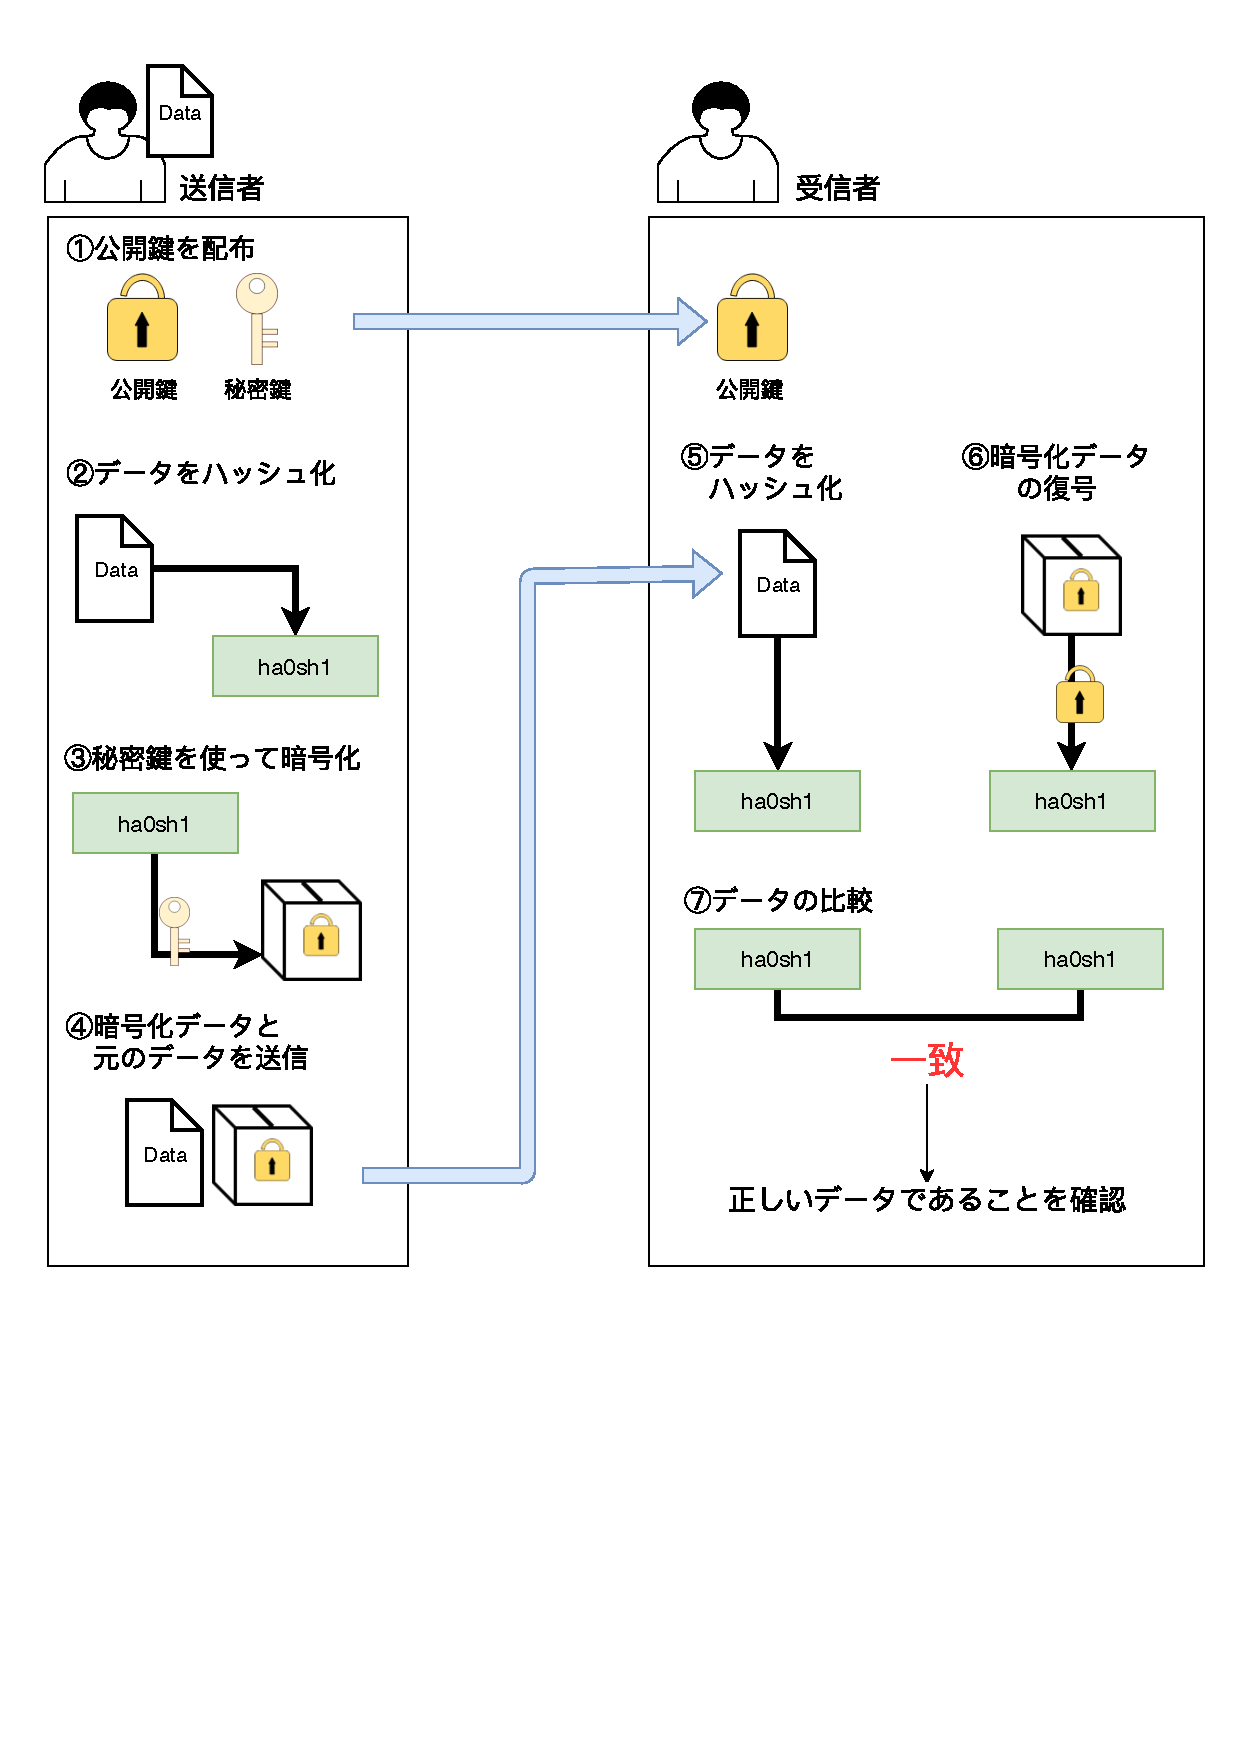
\includegraphics[mediaboxonly=/CropBox,width=12cm]{shomei.pdf}
\caption{電子署名の流れ}
\label{fig:no}
\end{figure} 





\subsection{SSL暗号化通信}
共通鍵暗号方式は公開鍵暗号方式よりも負荷が小さいが,鍵の受け渡し時に傍受される危険性があった.
そこで鍵の受け渡し時に公開鍵暗号方式を用いることで安全性を確保したものがSSL暗号化通信である.

\subsubsection{SSL暗号化通信の仕組み}

SSL暗号化通信では最初にユーザがサーバに接続要求を行い,送られてくるSSLサーバ証明書によって安全性を確認する.
安全性を確認したら,共通鍵を公開鍵暗号通信を使ってサーバに送ることで安全に共通鍵の受け渡しを行うことができる.




\begin{figure}[H]
\centering
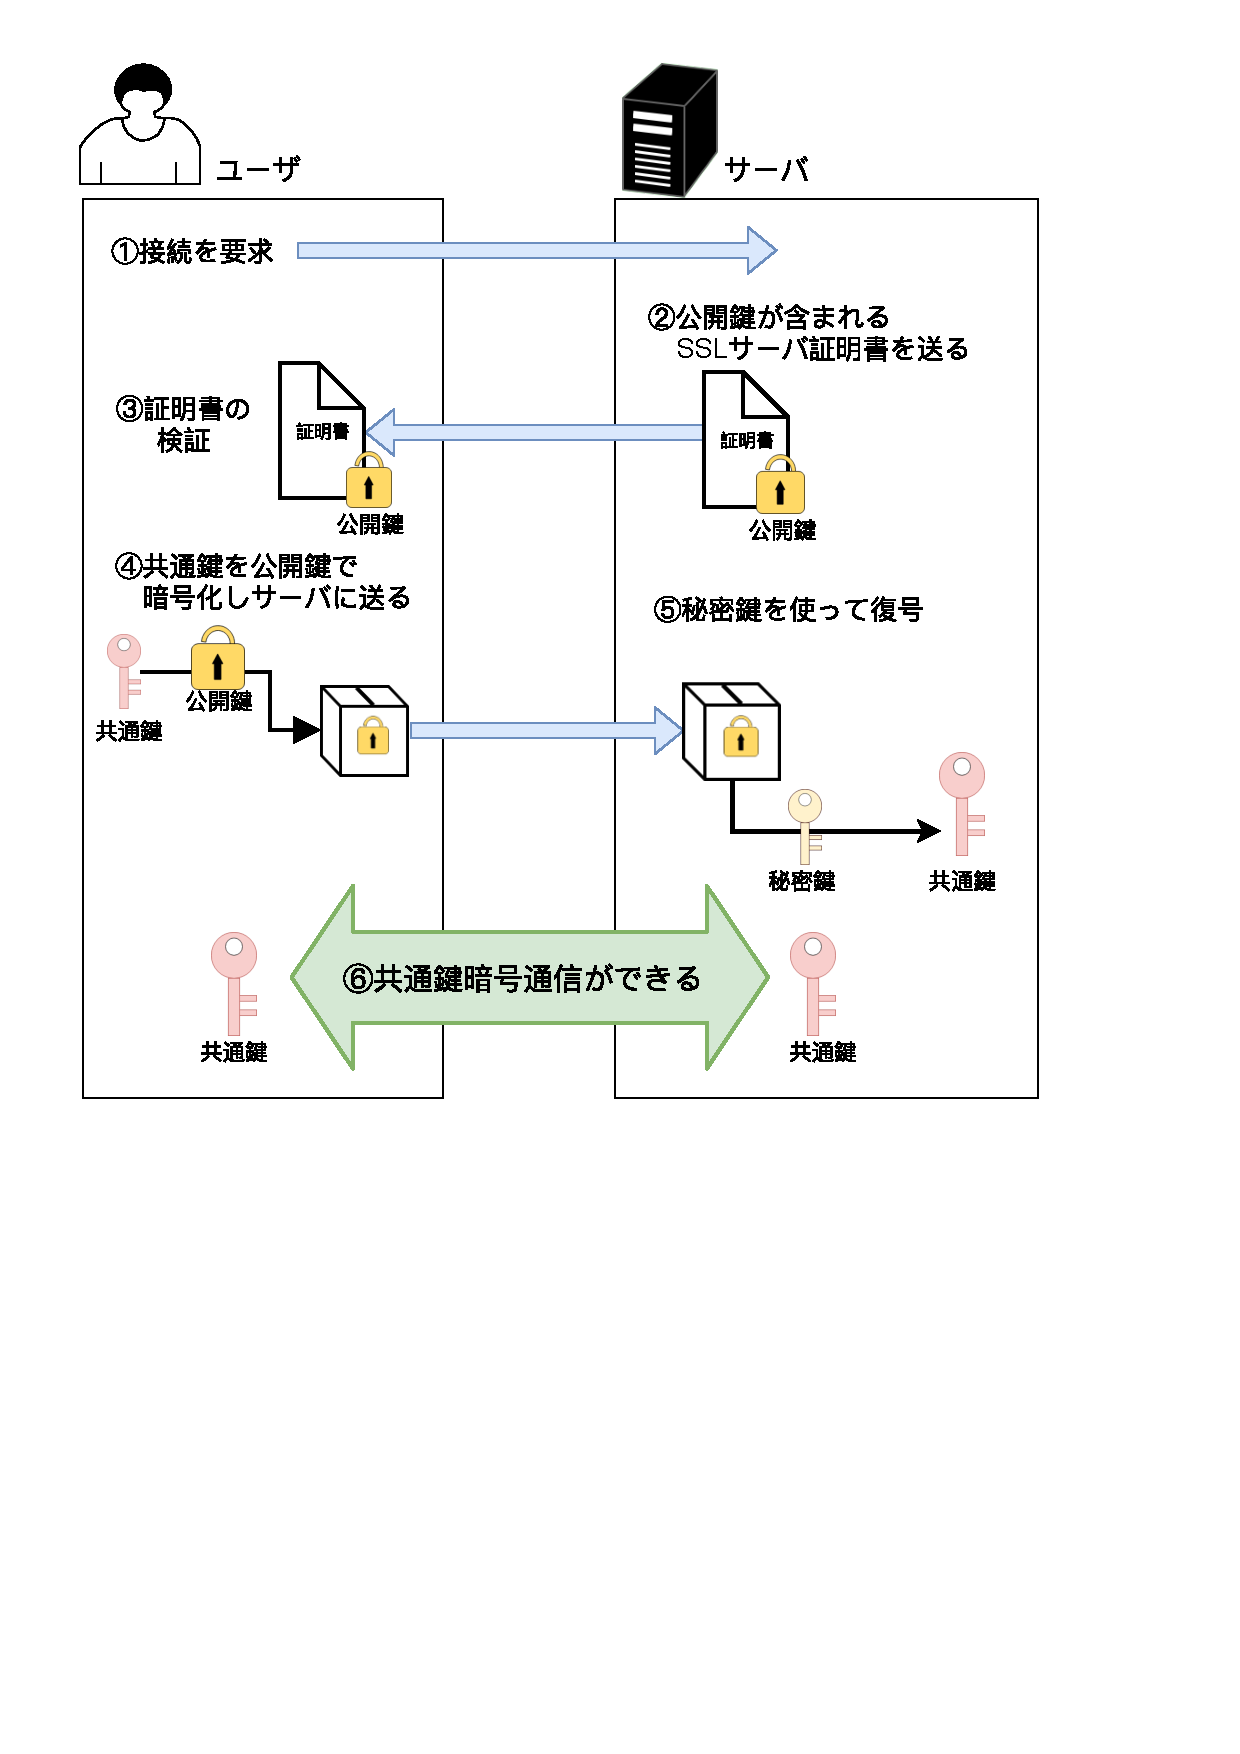
\includegraphics[mediaboxonly=/CropBox,width=14cm]{SSL.pdf}
\caption{SSL暗号化通信の流れ}
\label{fig:no}
\end{figure} 



\newpage
\section{ブロックチェーン}
ブロックチェーンとは,2009年にSatoshi Nakamoto氏の論文\cite{satoshi}で提唱された仮想通貨であるビットコインの根幹技術として生まれた分散型台帳システムである.


\subsection{ブロックチェーンの特徴}

取引を記録する台帳の1ページをブロックという.
ブロックチェーンはインターネット上の複数のコンピュータでお互いに取引の記録を共有し,検証しながら正しい記録の入ったブロックを鎖のように繋げていく.

\begin{figure}[H]
\centering
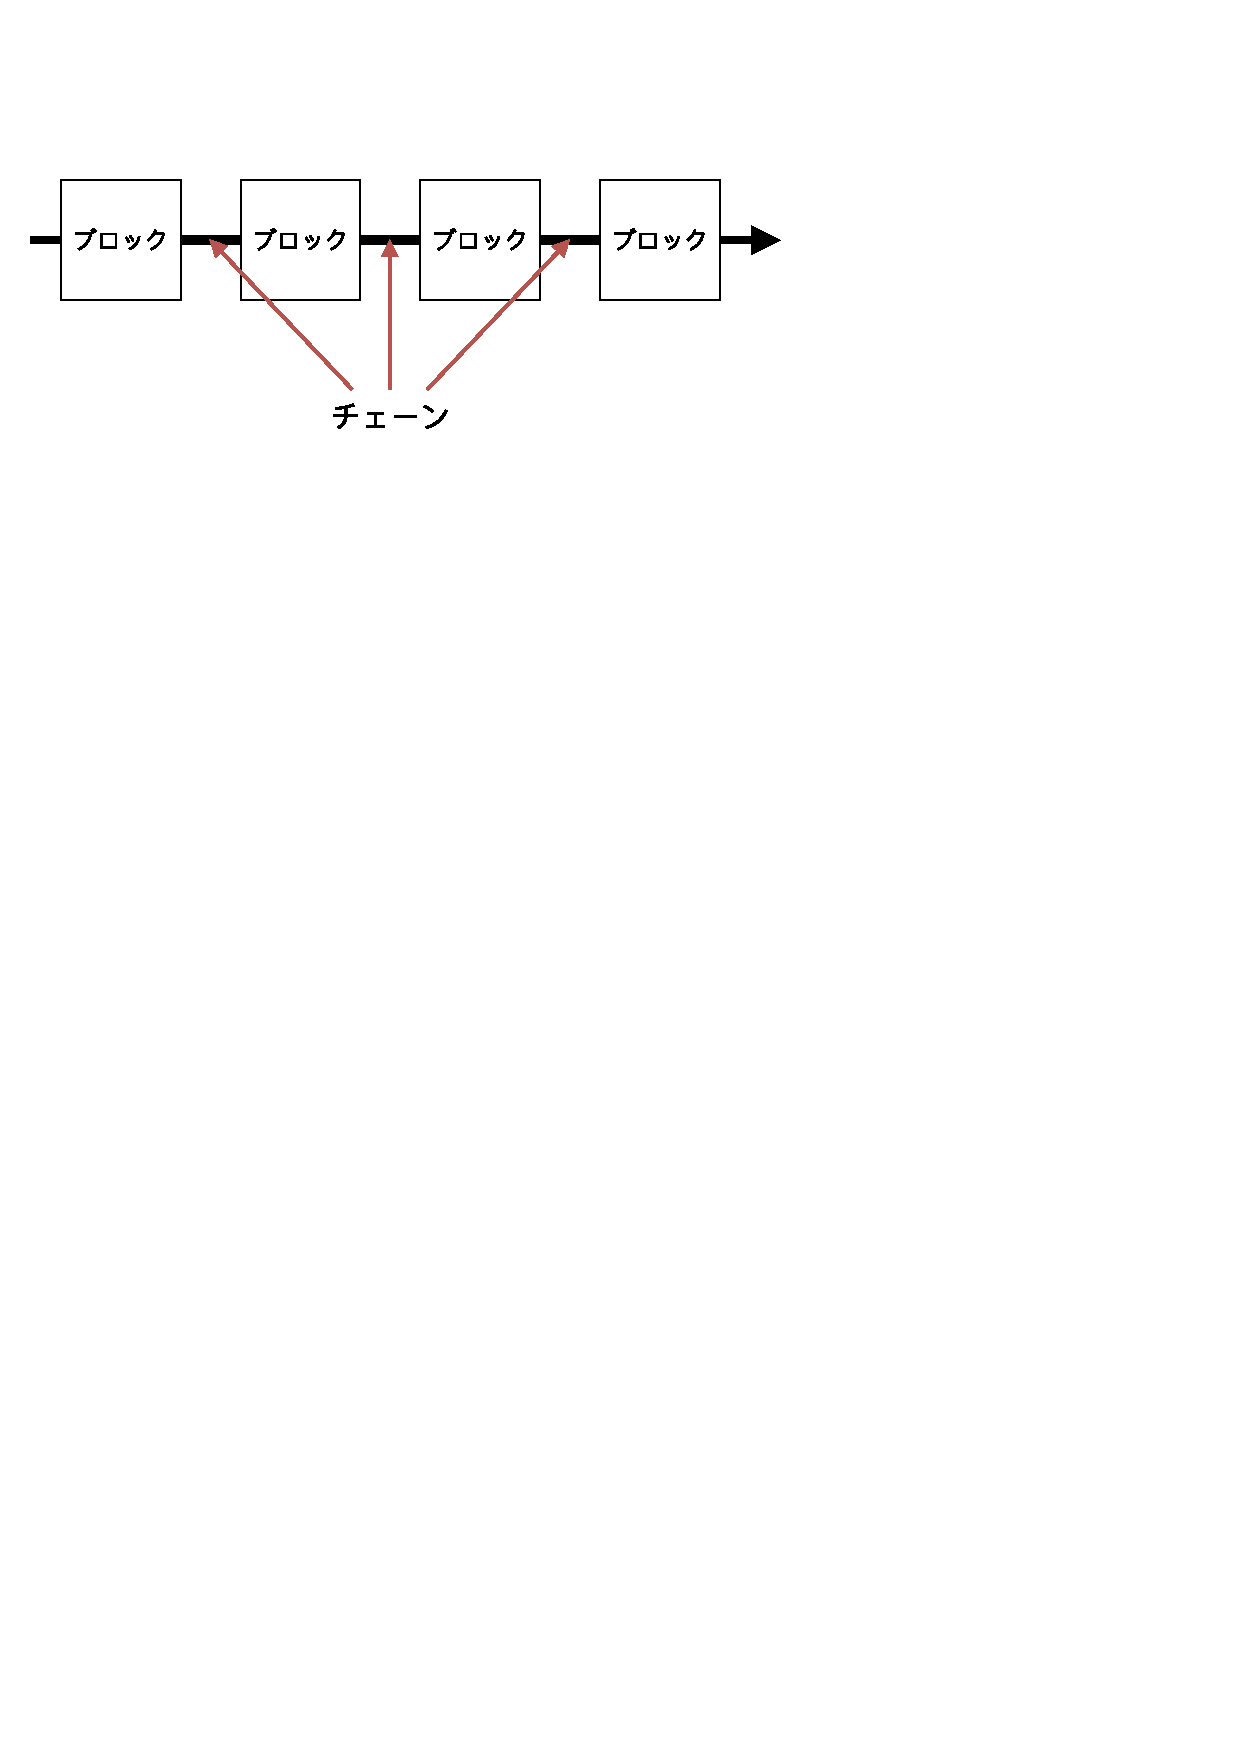
\includegraphics[mediaboxonly=/CropBox,width=11cm]{block1.pdf}
\caption{ブロックチェーンとは}
\label{fig:no}
\end{figure} 


\subsubsection{改ざんへの耐性がある}
ブロックチェーンの各ブロックはハッシュ関数によって繋がれている.ハッシュは不可逆性を持っており,ハッシュ値から元のデータを復元することはできない.ブロックチェーンでは複数の取引データがハッシュ化によって1ブロックにまとめられ,次のブロックに追加される.そのため過去のブロックを改ざんすると次のブロックとの整合性が取れなくなるため改ざんが困難である.


\newpage
\subsubsection{P2P分散型システム}
ブロックチェーンはP2P(Peer to Peer)を用いて取引データをやりとりしている分散型のシステムである.
P2Pは特定の管理者がサーバを管理するクライアント・サーバ型とは違い,各ノード間で対等に直接通信を行い,ネットワークを形成するネットワークである.
\begin{figure}[H]
\centering
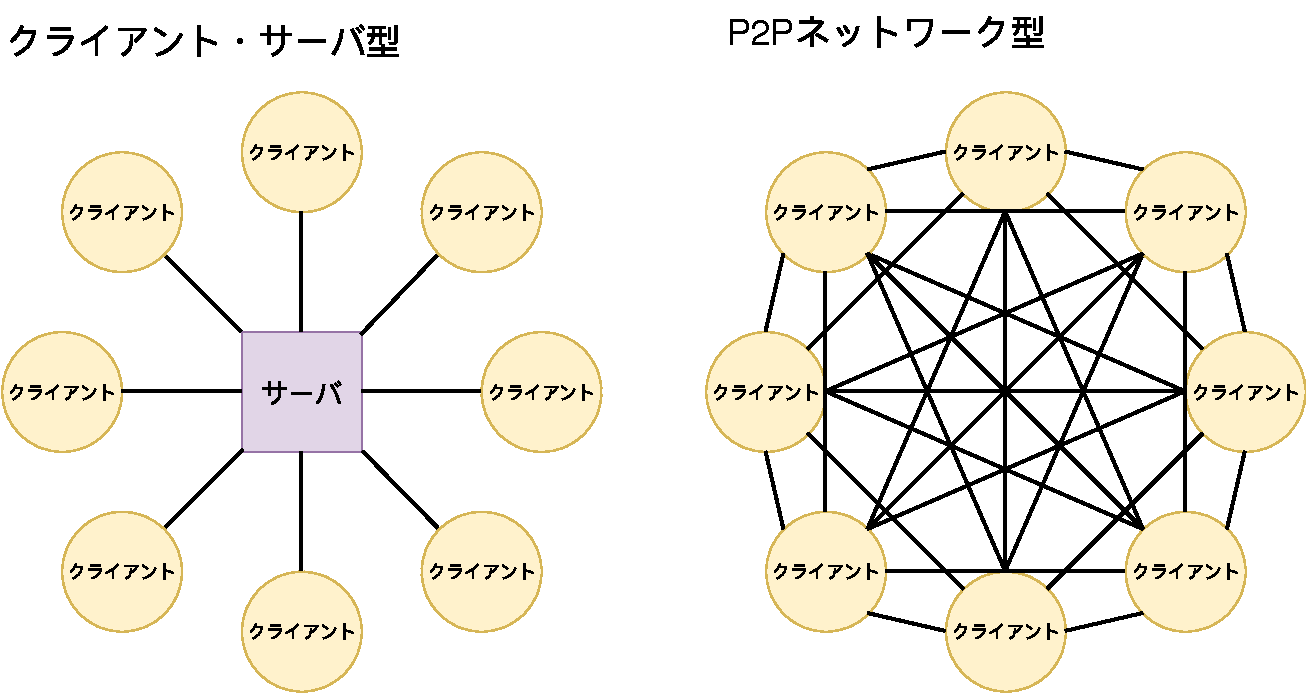
\includegraphics[width=13cm]{P2P.pdf}
\caption{クライアント・サーバ型とP2Pネットワーク型の違い}
\label{fig:no}
\end{figure} 



ブロックチェーンはP2Pネットワーク型であるため,データをまとめて記録したり,管理をしている機関のない非中央集権的なシステムとなっている.そのため一部のコンピュータに障害が発生してもシステムを維持することができる.

\subsubsection{ユーザとブロックチェーン間での通信}
ユーザとブロックチェーン間での通信には公開鍵暗号とハッシュを用いた電子署名の技術が使われる.
取引記録をハッシュ化したものを取引記録と一緒にブロックチェーンに送ることで,取引をしたユーザが本人であることを確認している.




\subsubsection{コンセンサスアルゴリズム}
チェーンにブロックを追加するにあたって,参加しているノードによる承認手続が必要となる.
ブロックチェーンでは管理者がいないため「不正」か「正当」の振り分けを,参加しているノードがある一定の条件のもとで行っている.またその一定の条件を満たしたノードが新たなブロックを作成する.

\subsection{仮想通貨とは}
一般的にはネットワーク上で電子的な決済の手段として流通しているが,法定通貨のように特定の国家による裏付けのないものである.ただし様々な種類の仮想通貨があり,定義や分類などは一様ではない.




\newpage
\subsection{コンセンサスアルゴリズムによるブロックチェーンの分類}
\subsubsection{Proof of Work(PoW)}
PoWではネットワークに参加しているノードは一番最初にnonceと呼ばれる値に当てはまる解を探す.このnonceを探す作業を採掘(マイニング)と呼ぶ.
採掘に成功したノードはブロックを作成し,ブロックチェーンをつなげる権利を得ることができる.

ビットコインではこのPoW方式が採用されている.
ビットコインの採掘では報酬として計算量に応じたビットコインをもらうことができる.\\

PoWの問題点としては総計算能力の過半数を占めるノードを用いることで虚偽のブロックを有効にすることができる51%問題がある.またPoWで報酬を得るためには高性能のコンピュータを常に起動して計算作業をさせる必要があり,無駄に電気コストがかかるという欠点もある.\\

\subsubsection{Proof of Stake(PoS)}
PoSでもブロック追加のためにはハッシュ関数等の計算による解が必要となるが,PoWでは計算量に応じた報酬を与えていたのに対し,仮想通貨の保有量に応じた報酬が与えられる.これはPoWの採掘に対し,鋳造(minting, forge)と呼ばれる.

またPoSではPoWと違い,計算量で争うことがなくなるため,PoWに比べ必要な電気コストが大幅に減らすことができる\cite{shu}.

PoWで51%攻撃をするためには膨大な計算能力を保有する必要があったが,PoSでは仮想通貨の総発行枚数の51%以上を保有する必要があり,PoWよりもコストがかかる.また自分が多く保有している通貨に攻撃を仕掛けるため,攻撃者にとってはメリットがあまりない.\\


しかしPoSでは通貨を保有することで報酬がもらえるという仕組みのため,通貨に必要な流動性が低くなってしまうという問題や流動性が低くなることで,仮想通貨の価格が低いときに大量に保有した人に報酬が集まり,貧富の差が広がるという問題がある.

\subsubsection{Proof of Importance(PoI)}

PoIでは参加者の重要度によって発言権が付与される.重要度は仮想通貨の保有量と取引(仮想通貨の流動性を高めたか)によって決められる.
PoSでは富裕層が有利になるというデメリットがあったが,PoI方式では流動性が高まるため,貧富の差が極端に広がることがない.PoIの仕組みによって報酬を得ることをハーベスティング(収穫)と呼ぶ.\\

しかしハーベスティングに参加するためには一定量の仮想通貨を保有する必要があり,PoSほどではないが富裕層が力を持つのではないかという懸念がある.



\newpage
\subsection{Proof of Workにおけるブロックチェーンの仕組み}
\subsubsection{ブロックに含まれるデータ}
ブロックにはハッシュ化した前の取引データの入ったブロック,取引データ,nonceが入っている.

\begin{figure}[H]
\centering
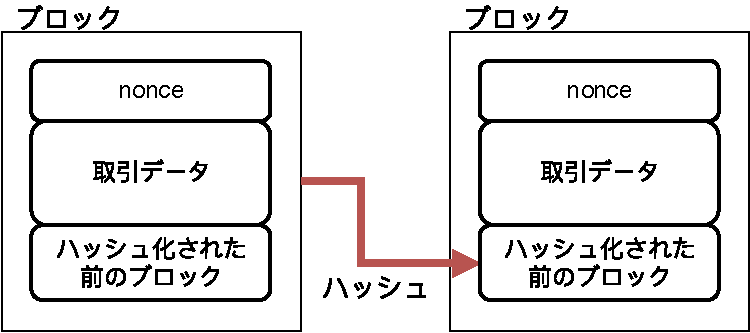
\includegraphics[width=11cm]{block2.pdf}
\caption{ブロックに含まれるデータ}
\label{fig:no}
\end{figure} 


\subsubsection{nonceの計算}
nonceは一定の長さの任意の値である.
nonceに数字を入れていき,ハッシュ化されたブロックの頭に0が一定数続くときにnonceを確定する.

ハッシュの元データは復元することができないため,nonceは総当たり的に探していくことになる.

\begin{figure}[H]
\centering
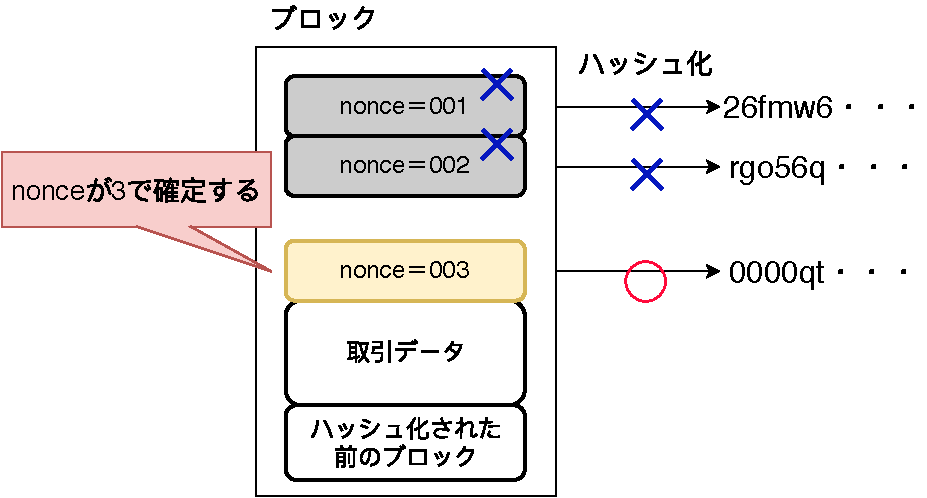
\includegraphics[width=14cm]{nonce.pdf}
\caption{nonceの計算}
\label{fig:no}
\end{figure} 

そのためデータが改ざんされると,改ざんされたブロック以降のnonceを全て総当たり的に探し直すこととなるためブロックチェーンが短くなる.ブロックチェーンが分岐したときは最も長いブロックチェーンのみを有効とするというルールがあるため,昔のブロックの改ざんほど難しくなる.

\begin{figure}[H]
\centering
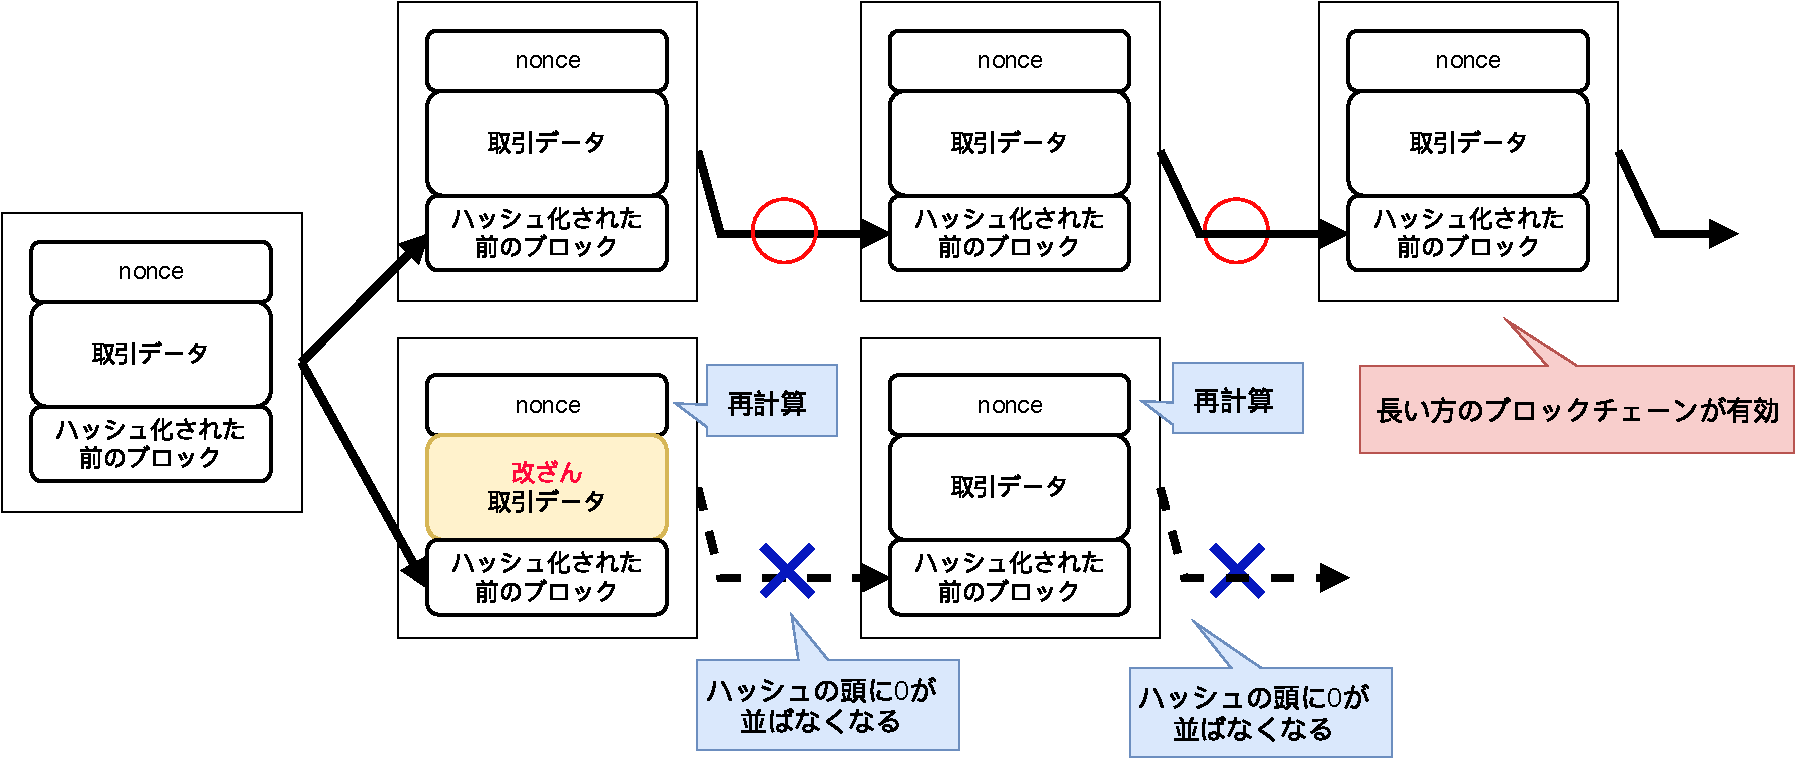
\includegraphics[width=14cm]{blockk.pdf}
\caption{改ざんを防ぐ仕組み}
\label{fig:no}
\end{figure} 

\newpage
\section{本研究で提案する仮説}
積み上げ型教科が苦手な学生は特定の箇所が苦手なのではなく,「どこがわかっていないのかもわからない」「そもそもいま何を教えられているかもわからない」など根本的な部分で躓いていて,
その原因として,前提知識には単元の学習目的が主単元で利用することとなっている単元が存在することだと考えた.
このことから以下の問題が起こると考える.

\begin{itemize}
\item 学習の目的がわかりづらい\\

このような単元では問題を解くことが目的となっており,学習する単元の具体的なイメージができないことが問題であると考えた.
そこで問題を解くことを目的にするのではなく,その技術を使って何ができるかを意識することが,理解の促進につながると考えた.


\item どの単元の知識を使えばいいかがわかりづらい\\
複数の前提単元を用いることで,学習内容がどちらの単元のものであったかなど混乱する学生がいると考えた.
そこで主単元の概要をあらかじめ学習し,複数の前提単元がどのように使われているかを明確にすることで,理解の促進につながると考えた.

\end{itemize}

このことから「主単元の概要をあらかじめ学習することで,前提単元の理解を促進することができる」という仮説を立てた.


\newpage
\section{実験}
本章では,提案した仮説が正しいことを証明するために実験を行う.以下で実験方法の解説を行う.
\subsection{実験目的}
本研究で提案した「主単元の概要をあらかじめ学習することで,前提単元の理解を促進することができる」という仮説の検証をすることを目的とする.

\subsection{実験方法}
\subsubsection{実験期間}

情報数学応用の講義にて3週かけて行う.

1週目:平成30年11月16日

2週目:平成30年11月30日

3週目:平成30年12月7日


\subsubsection{実験方法}

Aクラスでは仮説を用いない講義を行い,Bクラスでは仮説を用いた講義を行う.最後に両クラスで同一の小テストを行い,点数の比較と分析を行う.
また小テストと同じ用紙にて比較対象を同条件にするためのアンケートを行う.

(1)講義スケジュール

実験を行う講義は図\ref{fig:timeline}のように行う.
仮説を用いないAクラスでは最初に暗号とハッシュについて学習した後に,ブロックチェーンについて学習する.
仮説を用いたBクラスでは最初に暗号とハッシュを前提知識とするブロックチェーンの概要について学習した後に,暗号とは負について学習する.

\begin{figure}[H]
\centering
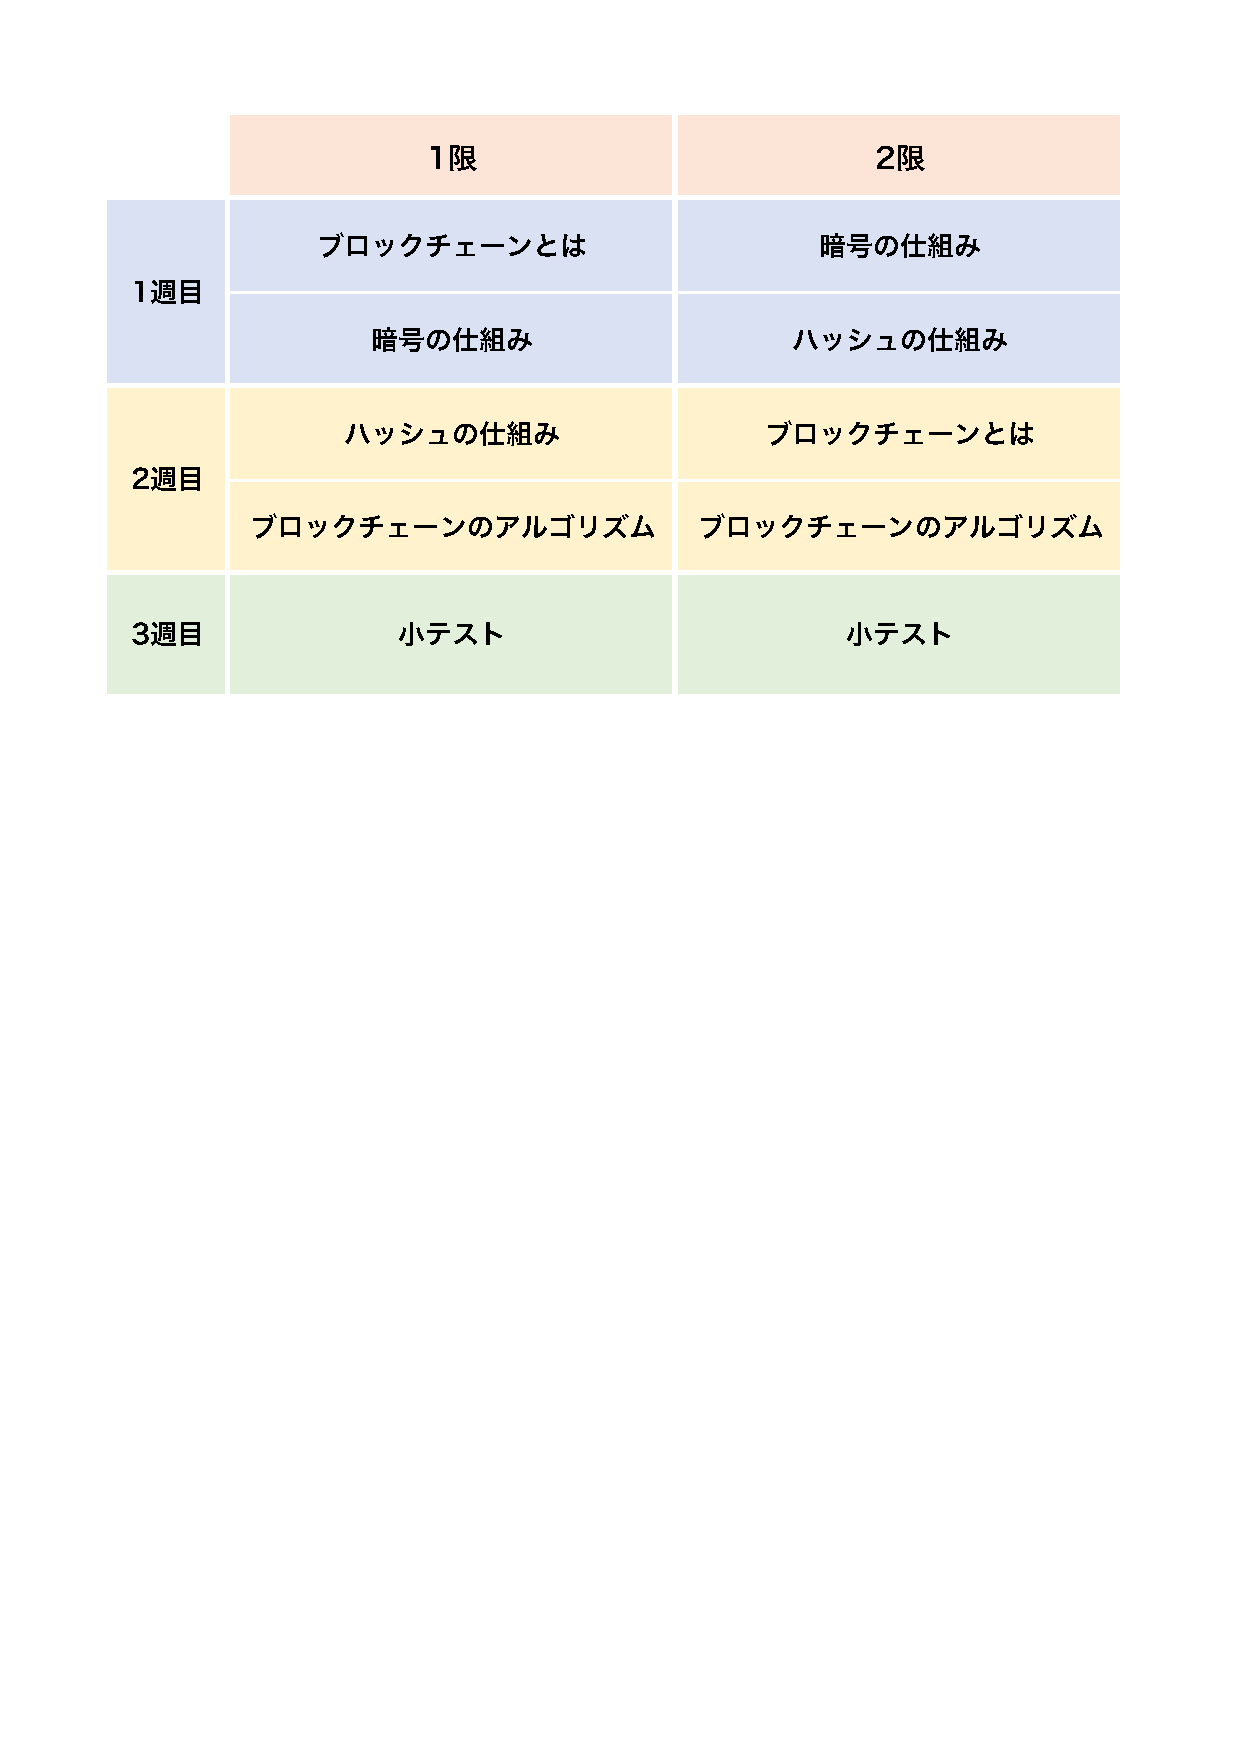
\includegraphics[mediaboxonly=/CropBox,width=10cm]{timeline.pdf}
\caption{講義スケジュール}
\label{fig:timeline}
\end{figure} 

(2)アンケートについて

アンケートにて「ブロックチェーンについて講義を受ける前に学習したことがあるか」について「はい」「いいえ」の二択で聞いた.
「はい」と答えた学生は仮説の「あらかじめ内容を理解する」に該当するが,人数に偏りができることと,元の知識により高得点を取る可能性が高いことから,比較の対象とはせず参考程度に留める.

またアンケート未回答の学生も比較の対象としないこととする.
\\


(3)小テスト内容

小テストでは以下の内容を問う.

\UTF{2460}RSA暗号の特徴

\UTF{2461}ハッシュと暗号の違い

\UTF{2462}ブロックチェーンの仕組み

点数配分は\UTF{2460}+\UTF{2461}で5点,\UTF{2462}で5点の合計10点とする.\\


(4)評価方法について

「前提単元」「主単元」「合計」の3つの観点で点数を比較する.
「前提単元」は \UTF{2460}RSA暗号の特徴 \UTF{2461}ハッシュと暗号の違い,「主単元」は \UTF{2462}ブロックチェーンの仕組み,「合計」は小テスト全体の点数(\UTF{2460}+\UTF{2461}+\UTF{2462})について平均点や偏差値を比較する.
また元の学力の差を考慮して,中間試験の偏差値との差を比較する.

\subsubsection{実験対象}

千葉工業大学 情報科学部 情報ネットワーク学科の学生のうち

2018年後期に開講された情報数学応用の受講者

Aクラス76名,Bクラス76名,計152名とする.\\

ただし複数回の講義を用いての実験であるため,比較や分析に使用するデータは小テスト受験者のみである.
またアンケートの結果,受講前にブロックチェーンを学習してことがない学生で,中間試験を受験している学生を比較と分析の対象とする.





\newpage
\section{実験結果}
\subsection{分析対象者に関するアンケートの結果}
「ブロックチェーンについて講義を受ける前に学習したことがあるか」という質問の結果は表\ref{fig:ank}のようになった.\\


\begin{table}[H]
\centering
\caption{アンケート結果}
\scalebox{1.2}{
\begin{tabular}{|c|c|c|}
\hline
\multicolumn{1}{|l|}{} & \multicolumn{1}{l|}{Aクラス} & \multicolumn{1}{l|}{Bクラス} \\ \hline
学習したことがない              & 60                      & 56                      \\ \hline
学習したことがある              & 4                       & 4                       \\ \hline
アンケート未回答               & 3                      & 2                       \\ \hline
小テスト未受験                & 9                      & 14                       \\ \hline
\end{tabular}
}

\label{fig:ank}
\end{table}

またブロックチェーンを学習したことがない学生のうち,中間試験を受験した学生は表\ref{fig:ank2}の通りとなった.

\begin{table}[H]
\centering
\caption{中間試験の受験状況}
\scalebox{1.2}{
\begin{tabular}{|c|c|c|}
\hline
\multicolumn{1}{|l|}{} & \multicolumn{1}{l|}{Aクラス} & \multicolumn{1}{l|}{Bクラス} \\ \hline
受験した             & 59                      & 54                      \\ \hline
未受験              & 1                       & 2                       \\ \hline
\end{tabular}
}

\label{fig:ank2}
\end{table}

この結果より小テストの点数の比較はAクラスが59人,Bクラスが54人の計113人を対象として行う.

\newpage
\subsection{講義のわかりやすさに関するアンケートの結果}
\subsubsection{暗号}


「暗号の講義はわかりやすかったか」という質問の結果は図\ref{fig:anank}のようになった.

両クラス共にわかりやすいと答えた学生が約60%となり,とてもわかりやすいと答えた学生と合わせて約80
%という結果となった.\\
\begin{figure}[H]
\centering
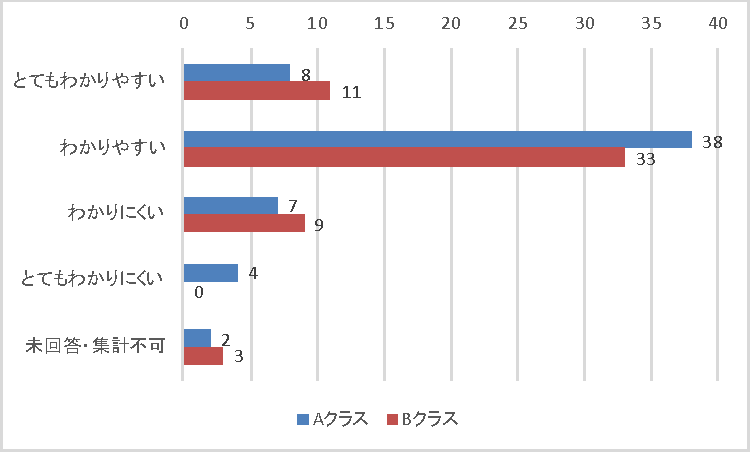
\includegraphics[width=12cm]{anka1.pdf}
\caption{暗号の講義についてのアンケート結果}
\label{fig:anank}
\end{figure}

\newpage
\subsubsection{ハッシュ}

「ハッシュの講義はわかりやすかったか」という質問の結果は図\ref{fig:hashank}のようになった.

両クラス共に「わかりにくい」と答えた学生の割合が一番高く,
「わかりやすい」と答えた学生の割合が次に高いという結果になった.
また「とてもわかりにくい」と答えた学生はAクラスでは2%,Bクラスでは0%となり,
暗号の講義と比べ両クラス共にわかりにくいと感じる学生が多いという結果になった.\\

\begin{figure}[H]
\centering
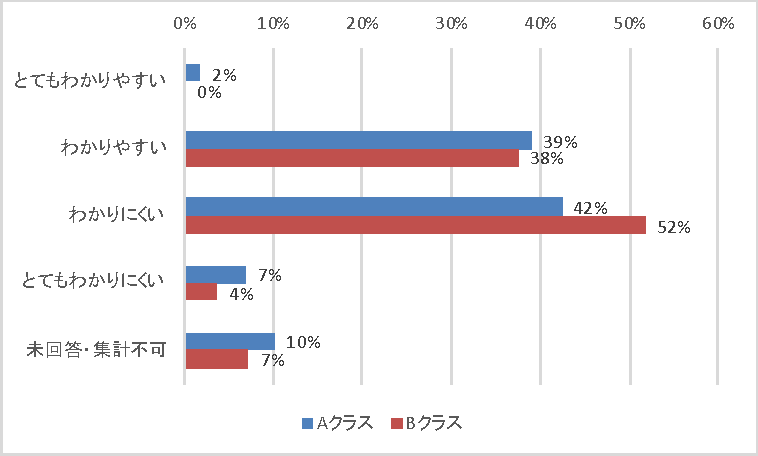
\includegraphics[width=12cm]{ankh1.pdf}
\caption{ハッシュの講義についてのアンケート結果}
\label{fig:hashank}
\end{figure}


\newpage
\subsubsection{ブロックチェーン}

「ブロックチェーンの講義はわかりやすかったか」という質問の結果は図\ref{fig:blockank}のようになった.

両クラス共に「わかりにくい」と答えた学生の割合が一番高く,
「わかりやすい」と答えた学生の割合が次に高くなり,ハッシュの講義に近い結果となった.\\
\begin{figure}[H]
\centering
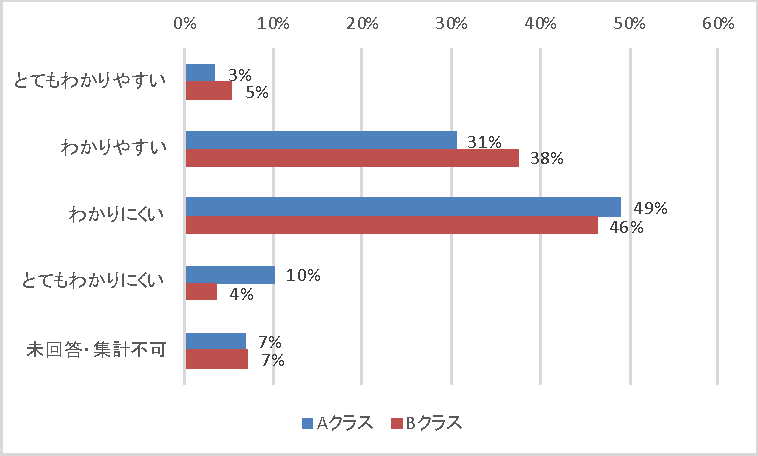
\includegraphics[width=12cm]{ankb1.pdf}
\caption{ブロックチェーンの講義についてのアンケート結果}
\label{fig:blockank}
\end{figure}





\newpage
\subsection{小テストの点数}
\subsubsection{前提単元}
前提単元は5点満点で,点数分布は図\ref{fig:zenten}のようになった.
Aクラスは4点の学生が一番多く約40%で,点数が低くなるにつれて割合が低くなった.
Bクラスは3点の学生が一番多く約30%で,Aクラスと同様に点数が低くなるにつれて割合が低くなったが,Aクラスよりも5点の学生の割合はわずかに高かった.また両クラス共に0点の学生はいなかった.

\begin{figure}[H]
\centering
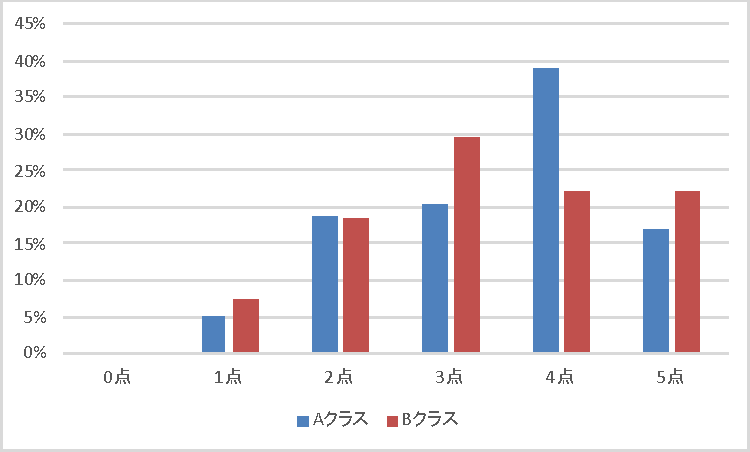
\includegraphics[width=12cm]{12test.pdf}
\caption{前提単元の点数分布}
\label{fig:zenten}
\end{figure} 

また前提単元の各クラスの偏差値と平均点は表\ref{fig:12ank}のようになった.
平均点はAクラスの方がわずかに高くなったが,中間試験の偏差値と比較したところほとんど差は見られなかった.\\
\begin{table}[H]
\centering
\caption{前提単元の偏差値と平均点}
\scalebox{1.1}{
\begin{tabular}{|c|c|c|c|c|}
\hline
\multicolumn{1}{|l|}{} & \multicolumn{2}{c|}{Aクラス} & \multicolumn{2}{c|}{Bクラス} \\ \cline{2-5}
                              & 偏差値 & 平均点  & 偏差値 & 平均点             \\ \hline
前提単元              & 50.4 & 3.4 /5  & 49.5 & 3.3 /5               \\ \hline
中間試験                       &50.6  & 29.4 /50 & 49.3 &     28.0 /50                  \\ \hline
\end{tabular}
}
\label{fig:12ank}
\end{table}





\newpage
\subsubsection{主単元}
主単元は5点満点で,点数分布は図\ref{fig:shuten}のようになった.
両クラス共に3点の学生が一番多く,4点以上の学生は人数が少なくなった.
Aクラスはまた両クラス共に0点の学生はいなかった.

\begin{figure}[H]
\centering
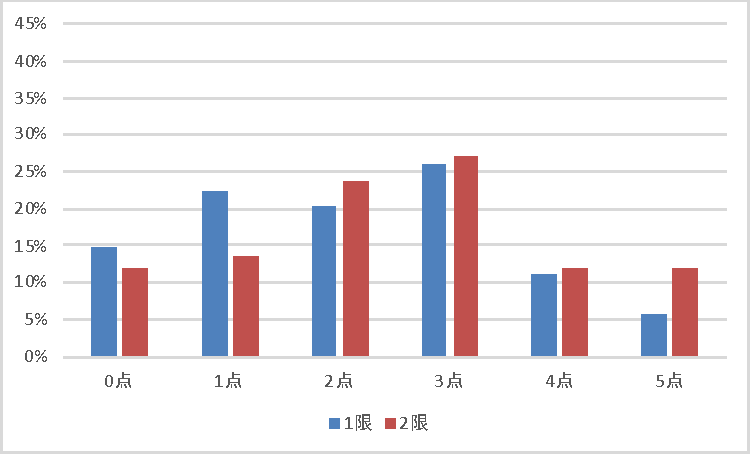
\includegraphics[width=12cm]{3test.pdf}
\caption{主単元の点数分布}
\label{fig:shuten}
\end{figure} 

また主単元の各クラスの偏差値と平均点は表\ref{fig:3ank}のようになった.
平均点はAクラスの方がわずかに高くなった.また中間試験の偏差値と比較してもAクラスの方が高くなった.\\

\begin{table}[H]
\centering
\caption{主単元の偏差値と平均点}
\scalebox{1.1}{
\begin{tabular}{|c|c|c|c|c|}
\hline
\multicolumn{1}{|l|}{} & \multicolumn{2}{c|}{Aクラス} & \multicolumn{2}{c|}{Bクラス} \\ \cline{2-5}
                              & 偏差値 & 平均点  & 偏差値 & 平均点             \\ \hline
主単元                       & 51.2 & 2.5 /5       & 48.7 & 2.1 /5                           \\ \hline
中間試験                       &50.6  & 29.4 /50 & 49.3 &     28.0 /50                  \\ \hline
\end{tabular}
}
\label{fig:3ank}
\end{table}



\newpage
\subsubsection{小テスト全体}
小テスト全体の点数は10点満点で,点数分布は図\ref{fig:allten}のようになった.
両クラス共に6点の学生が一番多く,点数が高くなるにつれて人数が少なくなった.
Aクラスは7点以上の割合が全体的に高く,Bクラスは4点以下の割合が全体的に高くなった.

\begin{figure}[H]
\centering
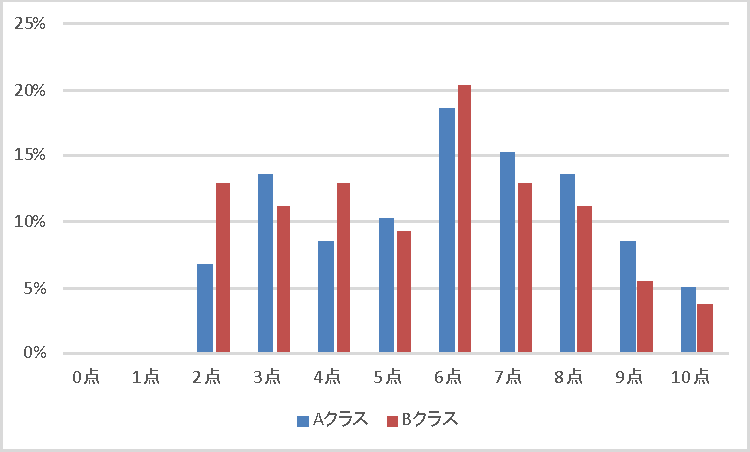
\includegraphics[width=12cm]{123test.pdf}
\caption{小テスト全体の点数分布}
\label{fig:allten}
\end{figure}

小テスト全体の偏差値と平均点は表\ref{fig:allank}のようになった.
平均点はAクラスの方がわずかに高くなった.また中間試験の偏差値と比較してもAクラスの方が高くなった.\\

\vspace{1zh}
\begin{table}[H]
\centering
\caption{小テストの偏差値と平均点}
\scalebox{1.1}{
\begin{tabular}{|c|c|c|c|c|}
\hline
\multicolumn{1}{|l|}{} & \multicolumn{2}{c|}{Aクラス} & \multicolumn{2}{c|}{Bクラス} \\ \cline{2-5}
                              & 偏差値 & 平均点  & 偏差値 & 平均点             \\ \hline
小テスト                       & 51.0 & 5.9 /10       & 48.9 & 5.6 /10                           \\ \hline
中間試験                       &50.6  & 29.4 /50 & 49.3 &     28.0 /50                  \\ \hline
\end{tabular}
}
\label{fig:allank}
\end{table}

 


\newpage
\section{考察}
今回の実験では仮説を証明することができなかった.
そこで実験方法に関する原因や改善点を以下のように考察した.

\subsection{スケジュール}
まず今回の実験は講義にて行った.一週目と二週目の間に休講日があり,時間が空いてしまったことから,講義外での勉強量が深く関係してしまい,講義での理解度が測ることができなかった可能性がある.そのため講義ではなく別の方法を用いて,期間を開けずに小テストまで終わらせることや,講義外での自習を行えない環境にするなど,別の実験方法で行うべきである.

また講義と小テストを別日で行ったため講義を欠席して小テストのみ受けた学生などの考慮が甘く,講義と小テストを受けた学生のみで実験を行うべきであった.





\subsection{試験問題}

図\ref{fig:test5}で示すように「前提単元」「主単元」の問題の難易度に差ができてしまった.簡単な問題は講義から時間が経っていても解けるが,難解な問題は内容を忘れやすく,前述した休講日も合間って時間が経っているクラスの点数に影響が出ている可能性がある.そのため前提単元と主単元の問題難易度を合わせる必要がある.
\begin{table}[H]
\centering
\caption{前提知識を用いた単元の平均点の比較}
\scalebox{1.1}{
\begin{tabular}{|c|c|c|}
\hline
\multicolumn{1}{|l|}{} & \multicolumn{1}{l|}{Aクラス} & \multicolumn{1}{l|}{Bクラス} \\ \hline
前提単元                       & 3.44      & 3.33                           \\ \hline
主単元                           & 2.49      & 2.13                        \\ \hline
\end{tabular}
}
\label{fig:test5}
\end{table}



\subsection{授業の選定}
今回の実験で前提単元として扱った暗号やハッシュには他の講義で扱った行列や誤り検出訂正などの前提知識が必要である.元の学力の差を考慮するために中間試験の点数との比較を行ったが,本実験に関係する知識の元の学力を測るものとは言えなかったため点数にズレが生じてしまった可能性がある.

また仮説を提唱した理由の一つが「前提単元の目的をはっきりさせることで理解が促進できる」ことであったが,今回の実験で用いた暗号技術は実用例が割と身近にあり,ブロックチェーンを目的にするよりもわかりやすいと感じる学生が多かったと考えた.



\newpage
\section{結言}
各塾の調査では中学,高校で学習する科目の中で数学と英語は苦手になりやすいと言われている\cite{1}.この2科目の共通点である積み上げ型教科という点に注目した.積み上げ型教科とは既に学習した知識を使うことを前提として授業を行う教科である.本研究では前提知識となる単元を「前提単元」,前提知識を用いて学習を行う単元を「主単元」と称した.前提単元には学習目的が主単元で利用することになっているものがあり,このような単元は学習目的や実用例などのイメージがしづらく,理解の妨げになっていると考えた.また前提単元が理解できないと主単元にまで影響を及ぼしてしまい,理解できない単元が増えるため,苦手な教科になってしまう.

そこで本研究では積み上げ型教科での理解力向上を目的として,「学習する単元を前提知識とする単元の概要をあらかじめ説明することで,内容の理解を促進することができる」という仮説を立て,仮説の証明を目指した.
しかし今回行った実験のみでは仮説が正しいことを証明することができなかった.しかし実験方法に多くの改善点が見つかったため,仮説が間違っていると断定することもできないという結果になった.

\newpage
\section{謝辞}
本研究の遂行および本論文の作成にあたり,多くの御助言と御指導いただきました須田宇宙准教授に深く感謝の意を表します.
また実験に協力していただいた情報数学応用の受講者に深く感謝の意を表します.


\newpage
\begin{thebibliography}{9}
\bibitem{1}
ベネッセ教育情報サイト:“教科学習が不得意と感じている高校生が9割!そのほとんどが英語と数学に偏るのにはある理由が”, \url{https://www.benesse.jp/kyouiku/201603/20160329-3.html}, (参照 2018-8-14)
\bibitem{satoshi}
Satoshi Nakamoto, “Bitcoin:A Peer-to-Peer Electronic Cash System”,2009年
\bibitem{shu}
 ”コンセンサスアルゴリズムとは?「PoW・PoS・PoI」の種類と違いを解説”.はじめてのビットコイン.\url{https://www.newscrypto.jp/articles/2612},(参照 2019-1-9)
\end{thebibliography}

\end{document}
